\chapter{سرعة المجموعة، والاستبعاد الفرميوني، وبحر ديراك}

\section{سرعة الطور وسرعة المجموعة}

\begin{classroomqa}
\lecturetimestamp{00:00:07}
\audiencequestion{ما المقصود بسرعة المجموعة وسرعة الطور؟}
\lecturerresponse{تتبع سرعة الطور نقطة ذات طور ثابت في موجة مستوية. وهي عمومًا لا تصف حركة جسم قابل للقياس. وتتبع سرعة المجموعة غلاف حزمة موجية، وهي السرعة المرتبطة بالجسيمات والإشارات وتدفق الاحتمال.}
\end{classroomqa}

ابدأ بموجة مستوية،
\begin{equation}
\psi(x,t)=e^{i(kx-\omega t)},
\end{equation}
أو بصورتها الحقيقية،
\begin{equation}
\psi(x,t)=\sin(kx-\omega t).
\end{equation}
تتحرك قمة أو قاع أو أي نقطة أخرى ذات طور ثابت بحيث
\begin{equation}
kx-\omega t=\text{constant}.
\end{equation}
وباختيار الثابت صفرًا للتيسير نحصل على
\begin{equation}
x=\frac{\omega}{k}t,
\qquad
v_{\mathrm{phase}}=\frac{\omega}{k}.
\end{equation}
وبما أن \(\omega=2\pi/T\) و\(k=2\pi/\lambda\)،
\begin{equation}
v_{\mathrm{phase}}=\frac{\omega}{k}=\frac{\lambda}{T}.
\end{equation}
وهذا هو ببساطة المسافة التي يتقدم بها طور معيّن خلال دورة واحدة.

بالنسبة إلى موجة Schr\"odinger غير نسبية، مع \(\hbar=1\)، تكون الطاقة والزخم هما \(\omega\) و\(k\)، ومن ثم
\begin{equation}
\omega(k)=\frac{k^2}{2m}.
\end{equation}
ولذلك فإن سرعة طورها هي
\begin{equation}
v_{\mathrm{phase}}=\frac{k}{2m}.
\end{equation}
غير أن السرعة المعتادة لجسيم زخمه \(k\) هي \(k/m\). وعدم التطابق بعامل اثنين هو أول تحذير من أن حركة طور الموجة المستوية ليست حركة الجسيم.

وثمة تحذير أشد. أضف الثابت نفسه \(C\) إلى كل تردد:
\begin{equation}
\omega(k)\longrightarrow \omega(k)+C.
\end{equation}
ويمكن أن يمثل هذا الثابت، على سبيل المثال، مساهمة مشتركة من طاقة السكون مثل \(mc_{\mathrm{light}}^2\)، لكن تسميته الدقيقة غير مهمة. وهنا تمثل \(C\) إزاحة في الطاقة، لا سرعة الضوء. وتتغير سرعة الطور إلى
\begin{equation}
v_{\mathrm{phase}}\longrightarrow
\frac{\omega(k)+C}{k}
=v_{\mathrm{phase}}+\frac{C}{k}.
\end{equation}
ومع ذلك فإن إضافة الثابت نفسه إلى كل طاقة لا تغيّر أي فرق في الطاقة، ومن ثم لا تغيّر شيئًا من الفيزياء غير النسبية.

يمكن رؤية ذلك مباشرةً في الدالة الموجية. اكتب حقل Schr\"odinger عامًا على هيئة مجموع أو تكامل لأنماط،
\begin{equation}
\psi(x,t)=\sum_k a_k e^{ikx}e^{-i\omega(k)t},
\end{equation}
مع حذف عوامل التطبيع. بعد الإزاحة،
\begin{align}
\psi(x,t)
&\longrightarrow
\sum_k a_k e^{ikx}e^{-i[\omega(k)+C]t}
\\
&=e^{-iCt}\psi(x,t).
\end{align}
يكتسب كل نمط الطور الزمني نفسه. ويكتسب الحقل المرافق الطور المعاكس، ولذلك
\begin{equation}
\begin{aligned}
\psi^*(x,t)\psi(x,t)
&\longrightarrow
e^{iCt}e^{-iCt}\psi^*(x,t)\psi(x,t)
\\
&=\psi^*(x,t)\psi(x,t).
\end{aligned}
\end{equation}
ويحدث الإلغاء نفسه في القيم المتوقعة. فالكمية التي تتغير عندما يُزاح مرجع الصفر للطاقة لا يمكن أن تكون سرعة الانتشار الفيزيائية لجسيم Schr\"odinger. ولذلك فإن سرعة الطور اصطلاحية جزئيًا.

يُمثَّل الجسيم الموضعي لا بموجة مستوية لا نهائية واحدة، بل بحزمة موجية. فالموجات المكوِّنة تتراكب تراكبًا بنّاءً في منطقة الحزمة وتراكبًا هدّامًا خارجها. ويمكن إيجاد حركة هذا النمط بالفعل من موجتين متقاربتين:
\begin{equation}
\psi(x,t)=
\sin(kx-\omega t)+
\sin(k'x-\omega't),
\end{equation}
حيث إن \(k'\) قريب من \(k\) و\(\omega'=\omega(k')\). ويقع موضع للتداخل البنّاء حيث يتفق طوراهما،
\begin{equation}
kx-\omega t=k'x-\omega't.
\end{equation}
وعليه
\begin{equation}
(k-k')x=(\omega-\omega')t,
\end{equation}
ويتحرك النمط المعزِّز وفقًا لـ
\begin{equation}
x=\frac{\omega-\omega'}{k-k'}t.
\end{equation}
وبأخذ حد الموجتين المتجاورتين نحصل على
\begin{equation}
x=\frac{d\omega}{dk}t,
\qquad
v_{\mathrm{group}}=\frac{d\omega}{dk}.
\end{equation}
وهذه هي سرعة الغلاف---أي التكتل الموضعي الناتج من تداخل الموجات المكوِّنة.

وبالنسبة إلى علاقة التشتت غير النسبية، مع تضمين الإزاحة الاعتباطية،
\begin{equation}
\omega(k)=\frac{k^2}{2m}+C,
\end{equation}
فإن سرعة المجموعة هي
\begin{equation}
v_{\mathrm{group}}
=\frac{d}{dk}\left(\frac{k^2}{2m}+C\right)
=\frac{2k}{2m}
=\frac{k}{m}.
\end{equation}
وقد اختفى الثابت الجمعي، والنتيجة هي بالضبط سرعة الجسيم الكلاسيكية.

\begin{classroomqa}
\lecturetimestamp{00:16:35}
\audiencequestion{هل يختفي عامل الاثنَين في سرعة المجموعة؟}
\lecturerresponse{نعم. إن اشتقاق \(k^2\) يعطي \(2k\)، وهذا يلغي الاثنَين في \(2m\). والنتيجة هي \(k/m\).}
\end{classroomqa}

وعليه فإن سرعة المجموعة هي السرعة الأوثق ارتباطًا بحركة الجسيم الكلاسيكية. وهي أيضًا السرعة ذات الصلة بانتشار حزمة موجية، وفي الظروف المعتادة المدروسة هنا، بانتشار الإشارات. ولا يلزم أن يكون لسرعة الطور أيٌّ من هذين المعنيين.

\subsection{الموجات النسبية عديمة الكتلة وذات الكتلة}

\begin{classroomqa}
\lecturetimestamp{00:17:47}
\audiencequestion{هل لهذا صلة بالادعاءات القائلة إن الضوء يمكن أن ينتقل أسرع من الضوء؟}
\lecturerresponse{لا. تثير تلك الادعاءات مسألة منفصلة. وهناك حساب ذو صلة يُظهر فعلًا أن طورًا يمكن أن يتحرك أسرع من الضوء بينما تظل سرعة المجموعة الفيزيائية دون سرعة الضوء، لكن هذا لا يصف إشارة تسبق الضوء.}
\end{classroomqa}

\begin{classroomqa}
\lecturetimestamp{00:18:05}
\audiencequestion{هل المثال ذو الصلة هو المثال المألوف الذي تتجاوز فيه سرعة الطور سرعة الضوء بينما تظل سرعة المجموعة دونها؟}
\lecturerresponse{نعم. يظهر النمط نفسه لموجة نسبية ذات كتلة غير صفرية، ويتبع مباشرةً من علاقة الطاقة--الزخم النسبية.}
\end{classroomqa}

ضع \(\hbar=c_{\mathrm{light}}=1\). والعلاقة النسبية هي
\begin{equation}
E=\sqrt{p^2+m^2},
\qquad
\omega(k)=\sqrt{k^2+m^2}.
\end{equation}
ومن المفيد أولًا تناول حالة انعدام الكتلة. عندما \(m=0\)،
\begin{equation}
\omega=|k|.
\end{equation}
وعلى الفرع المتجه يمينًا \(k>0\)، يكون \(\omega=k\)، ومن ثم
\begin{equation}
v_{\mathrm{phase}}=\frac{\omega}{k}=1,
\qquad
v_{\mathrm{group}}=\frac{d\omega}{dk}=1.
\end{equation}
وعلى الفرع المتجه يسارًا تكون لكلتا السرعتين الإشارة السالبة المناظرة. وفي كلتا الحالتين يكون مقدار السرعة هو سرعة الضوء. ولأن علاقة التشتت خطية على أيٍّ من الفرعين، فإن جميع مركبات فورييه على ذلك الفرع تتحرك بالسرعة نفسها.

أما لجسيم ذي كتلة مع \(k>0\)،
\begin{equation}
v_{\mathrm{phase}}
=\frac{\omega}{k}
=\sqrt{\frac{k^2+m^2}{k^2}}>1,
\end{equation}
في حين أن
\begin{equation}
v_{\mathrm{group}}
=\frac{d\omega}{dk}
=\frac{k}{\sqrt{k^2+m^2}}<1.
\end{equation}
وأما إذا كان \(k<0\) فإن كلتا السرعتين تعكسان الإشارة، بينما يخضع مقداراهما للمتباينات نفسها. وهكذا يمكن للطور أن يتحرك أسرع من الضوء بينما تتحرك الحزمة والجسيم والطاقة والإشارة أبطأ من الضوء. وبالنسبة إلى علاقة التشتت هذه تحديدًا ومع \(k\neq0\)،
\begin{equation}
v_{\mathrm{phase}}v_{\mathrm{group}}=1.
\end{equation}
وهذه العلاقة العكسية مصادفة ناتجة من علاقة التشتت ذات الجذر التربيعي، وليست خاصية عامة للموجات.

\begin{figure}
\centering
\includegraphics[width=0.72\textwidth]{lecture_05_figure_03.png}
\caption{علاقتا التشتت غير النسبية والنسبية، مع سرعة الطور \(\omega/k\) وسرعة المجموعة \(d\omega/dk\).}
\lectureframe{00:35:52}
\end{figure}

\begin{classroomqa}
\lecturetimestamp{00:23:41}
\audiencequestion{هل يرتبط التشتت بأن تعتمد سرعة الموجة على التردد؟}
\lecturerresponse{نعم. عندما تكون \(\omega(k)\) خطية، تكون لجميع مركبات فورييه سرعة المجموعة نفسها، ويمكن للحزمة أن تحتفظ بشكلها. وعندما تكون \(\omega(k)\) لاخطية، تتحرك المركبات بسرعات مختلفة، فتتشتت الحزمة ويتغير شكلها. ويكون الصوت منخفض التردد تقريبًا غير متشتت عندما يكون تردده متناسبًا تقريبًا مع عدد الموجة.}
\end{classroomqa}

وعادةً لا تحمل سرعة الطور إشارةً ولا طاقةً ولا تدفقًا للاحتمال. بل إن قيمتها العددية يمكن أن تتغير بإزاحة مرجع الصفر للطاقة. أما سرعة المجموعة فهي الحركة الفيزيائية ذات الصلة لحزمة ضيقة بما يكفي.

\begin{classroomqa}
\lecturetimestamp{00:25:14}
\audiencequestion{هل يمكن قياس سرعة الطور لفوتون؟}
\lecturerresponse{في الفراغ يخضع الفوتون لعلاقة تشتت خطية، لذلك تتطابق سرعتا الطور والمجموعة لديه، وتساويان كلتاهما سرعة الضوء. أما في وسط مادي فتتغير علاقة التشتت، ولا يلزم أن تتفق سرعتا الطور والمجموعة.}
\end{classroomqa}

\begin{classroomqa}
\lecturetimestamp{00:25:50}
\audiencequestion{هل يقتصر هذا النقاش على الحزم الموجية التي لا تتسع مع الزمن؟}
\lecturerresponse{لا تبقى الحزمة غير متسعة إلا عندما تشترك جميع مركبات فورييه فيها في سرعة واحدة، وهذا يقابل علاقة تشتت خطية على المدى المعني. ومع علاقة تشتت لاخطية تنفصل المركبات وتتسع الحزمة.}
\end{classroomqa}

الأسئلة المتعلقة بمخاريط الضوء والبنية السببية النسبية تتطلب أكثر من مجرد التمييز بين سرعة الطور وسرعة المجموعة، ولذلك تُترك منفصلة عن هذا الحساب.

\section{تناظر الانتقال وقوانين الانحفاظ}

تعطي أطوار الموجة المستوية نفسها عرضًا موجزًا لقوانين الانحفاظ. لنبدأ بانحفاظ الطاقة. فحقل الإفناء المؤثر في جسيم وارد طاقته \(\omega_j\) يساهم بعامل زمني
\begin{equation}
e^{-i\omega_j t},
\end{equation}
في حين أن حقل الخلق الذي يُنتج جسيمًا صادرًا طاقته \(\omega'_r\) يساهم بـ
\begin{equation}
e^{+i\omega'_r t}.
\end{equation}
ولعدة جسيمات واردة وصادرة، يكون حاصل ضرب هذه العوامل
\begin{equation}
\exp\!\left[
i\left(\sum_r\omega'_r-\sum_j\omega_j\right)t
\right].
\end{equation}
وإذا كان يمكن أن يقع التآثر في أي زمن وبالسعة نفسها، فإن السعة تتضمن تكاملًا على زمن التآثر:
\begin{equation}
\begin{aligned}
&\int_{-\infty}^{\infty}dt\,
\exp\!\left[
i\left(\sum_r\omega'_r-\sum_j\omega_j\right)t
\right]
\\
&\quad =2\pi\,
\delta\!\left(\sum_r\omega'_r-\sum_j\omega_j\right).
\end{aligned}
\end{equation}
وتقتضي دالة دلتا أن تساوي الطاقة الكلية الصادرة الطاقة الكلية الواردة. وثبات السعة عند كل زمن تآثر ممكن هو تناظر الانتقال الزمني، وهو ما ينتج انحفاظ الطاقة.

يعطي الانسحاب المكاني انحفاظ الزخم بالآلية نفسها. لننظر في اضمحلال فيزيائي من جسيم واحد إلى جسيمين، تختفي فيه جسيمة داخلة زخمها \(k\) وتظهر جسيمتان زخماهما \(k'_1\) و \(k'_2\). ويتضمن تآثر موضعي عند الموضع \(x\) حقلاً واحدًا للإفناء وحقلين للإنشاء،
\begin{equation}
\mathcal{O}(x)=\psi^\dagger(x)\psi^\dagger(x)\psi(x).
\end{equation}
ومع إغفال الاعتماد على الزمن وعامل التطبيع، تكون عوامل الأنماط ذات الصلة هي
\begin{align}
\psi(x)&\supset a_k e^{ikx},
\\
\psi^\dagger(x)&\supset a_{k'_1}^\dagger e^{-ik'_1x},
\qquad
\psi^\dagger(x)\supset a_{k'_2}^\dagger e^{-ik'_2x}.
\end{align}
وفي عنصر المصفوفة
\begin{equation}
\langle k'_1,k'_2|\mathcal{O}(x)|k\rangle,
\end{equation}
يزيل مؤثر الإفناء الجسيمة الداخلة، ويولِّد مؤثرا الإنشاء الجسيمتين الخارجتين. وبعد تنفيذ أفعال هذه المؤثرات، يكون العامل المعتمد على الموضع الذي يبقى هو
\begin{equation}
e^{-ik'_1x}e^{-ik'_2x}e^{ikx}
=e^{i(k-k'_1-k'_2)x}.
\end{equation}
ولأن أي موضع لا يتمتع بامتياز على غيره، نكامل على جميع مواضع الاضمحلال الممكنة:
\begin{equation}
\int_{-\infty}^{\infty}dx\,
e^{i(k-k'_1-k'_2)x}
=2\pi\delta(k-k'_1-k'_2).
\end{equation}
ولذلك تحقق السعة الباقية
\begin{equation}
k=k'_1+k'_2.
\end{equation}
وفي ثلاثة أبعاد يستخدم الحساب نفسه \(d^3x\) ومتجهات زخم غليظة ودالة دلتا ثلاثية الأبعاد. ولا يعتمد شيء في البرهان على وجود جسيمة داخلة واحدة فقط أو جسيمتين خارجتين فقط. ولأعداد جسيمات اعتباطية، ينتج عن التكامل على موضع التآثر المشترك
\begin{equation}
\delta^{(3)}\!\left(
\sum_j\mathbf{k}_j-\sum_r\mathbf{k}'_r
\right).
\end{equation}
وكون السعة متساوية عند كل موضع هو تناظر الانسحاب المكاني، وهو يعطي انحفاظ الزخم تمامًا كما أن تساوي السعة عند كل زمان يعطي انحفاظ الطاقة.

والمثال الثالث هو دوران طور عالمي،
\begin{equation}
\psi\longrightarrow e^{i\lambda}\psi,
\qquad
\psi^\dagger\longrightarrow e^{-i\lambda}\psi^\dagger.
\end{equation}
وتبقى سعة التآثر ثابتة عندما تلغي الأطوار التي تسهم بها حقول الإفناء والإنشاء بعضها بعضًا. وبالنسبة إلى حقل يحمل شحنة كهربائية، فإن تساوي الشحنة المنزوعة من الحالة الابتدائية والمُعادة في الحالة النهائية هو انحفاظ الشحنة. وهكذا توضّح الانسحابات الزمنية والانسحابات المكانية ودورانات الطور العالمية كيف تُشفِّر الحقول التي تُنشئ الجسيمات وتفنيها انحفاظ الطاقة والزخم والشحنة.

\begin{classroomqa}
\lecturetimestamp{00:37:52}
\audiencequestion{هل يعني التكامل على الفضاء التكامل على الأبعاد المكانية الثلاثة كلها؟}
\lecturerresponse{نعم. تولِّد التكاملات الثلاثة دالة دلتا لمركبات الزخم الثلاث، ولذلك تُحفَظ المركبات الثلاث كلها للزخم الكلي.}
\end{classroomqa}

\begin{classroomqa}
\lecturetimestamp{00:38:03}
\audiencequestion{هل يحدد هذا النموذج الاحتمالات النسبية للطرائق المختلفة لتوزيع الزخم المحفوظ؟}
\lecturerresponse{لا. فهذا التعبير البسيط يفرض مجموع الزخوم الخارجة، لكنه بخلاف ذلك محايد تجاه توزيعها. وتتطلب الاحتمالات النسبية معلومات ديناميكية إضافية.}
\end{classroomqa}

\begin{classroomqa}
\lecturetimestamp{00:39:04}
\audiencequestion{لماذا يختزل مجموع مؤثرات الإفناء إلى الحد المطابق للزخم المشغول؟}
\lecturerresponse{يعطي مؤثر الإفناء عندما يؤثر في نمط خالٍ المتجه الصفري. وإذا كانت الحالة تحتوي جسيمة واحدة في النمط \(k_0\) فقط، فإن كل حد ما عدا الحد ذي \(k=k_0\) ينعدم.}
\end{classroomqa}

فعلى سبيل المثال،
\begin{equation}
\sum_k a_k e^{ikx}|1_{k_0}\rangle
=e^{ik_0x}|0\rangle,
\end{equation}
وذلك مع إغفال عامل التطبيع: فجميع مؤثرات الإفناء المرتبطة بأنماط خالية تعطي المتجه الصفري.

\section{التعزيز البوزوني والاستبعاد الفرميوني}

تسمح البوزونات بأي عدد إشغال غير سالب في حالة أحادية الجسيم، وجبر مؤثرات إنشائها يفضّل فعلًا حالةً مشغولة سلفًا. وبالنسبة إلى نمط بوزوني واحد، تكتب اصطلاحات حالات العدد المطبَّعة تعزيز الإشغال على الصورة\footnote{تذكر المحاضرة تعزيز الإشغال بالجذر التربيعي؛ وهذه المعادلة المفهرسة هي صورته المعيارية في ترميز حالات العدد.}
\begin{equation}
a^\dagger|n\rangle=\sqrt{n+1}\,|n+1\rangle.
\end{equation}
افترض أن ذرة مثارة يمكنها أن تبعث فوتونًا إلى أنماط ممكنة كثيرة. وفي غياب فوتونات أخرى، تظهر الاتجاهات والزخوم المختلفة وفق توزعها الاحتمالي المعتاد. فإذا كان نمط معيَّن يحتوي مسبقًا على فوتونات كثيرة---كلها ذات الزخم والطاقة والتردد أنفسها---فإن الانبعاث إلى ذلك النمط يتعزز بعامل الجذر التربيعي للإشغال الموافق. فتضيف الذرة فوتونها على نحو تفضيلي إلى الحالة المشغولة بالفعل. وهذا هو الانبعاث المحفَّز، وهو تعبير ملموس عن تجمّع البوزونات.

تتصرف الفرميونات على النحو المعاكس. فلا يمكن لفرميونين متماثلين أن يشغلا الحالة الكمومية نفسها. وقد ظهر مبدأ الاستبعاد أولًا في الفيزياء الذرية، حيث لا يمكن لإلكترونين في ذرة واحدة أن تكون لهما الأعداد الكمومية نفسها، لكنه لا يقتصر على الذرات: فالفرميونات المتماثلة لا يمكنها أن تتقاسم حالة جسيم واحد كاملة في أي مكان.

يبدو توسيع الحقل في البداية مطابقًا تمامًا للتوسيع البوزوني. وفي صندوق محدود يمكن أن نكتب
\begin{equation}
\psi(x)=\sum_k A_k e^{ikx},
\qquad
\psi^\dagger(x)=\sum_k A_k^\dagger e^{-ikx}.
\end{equation}
وعند الزخم المتصل تتحول المجاميع إلى تكاملات. وتنتج الإشارة المعاكسة في الطور المكاني المرافق من الاقتران الهرميتي. وهذا الجزء من الصياغة غير نسبي؛ ولن تظهر الفرميونات النسبية إلا في النهاية.

ما زالت حالة الحقل تُسجَّل بعدد إشغال لكل نمط، لكن كل عدد الآن لا يمكن أن يكون إلا صفرًا أو واحدًا:
\begin{equation}
|n_{k_1},n_{k_2},\ldots\rangle,
\qquad n_k\in\{0,1\}.
\end{equation}
ولا توجد أنواع إضافية من الجسيمات النسبية يكون فيها، مثلًا، في كل حالة ثلاث جسيمات على الأكثر أو سبع جسيمات على الأقل. وإثبات أن إحصاءي البوزونات والفرميونات هما الإمكانان الوحيدان يتطلب ميكانيكا الكم مع النسبية الخاصة، وهو خارج نطاق المناقشة الحالية. أما هنا فالمهمة هي وصف الإمكان الفرميوني ونتائجه.

\subsection{حالة فرميونية واحدة}

لنركز على حالة أحادية الجسيم واحدة. فهي إما خالية، \(|0\rangle\)، أو مشغولة، \(|1\rangle\). ويكون فعل الإنشاء والإفناء كما يلي
\begin{align}
A^\dagger|0\rangle&=|1\rangle,
&
A^\dagger|1\rangle&=0,
\\
A|0\rangle&=0,
&
A|1\rangle&=|0\rangle.
\end{align}
والصفر غير المزيَّن في الطرف الأيمن هو المتجه الصفري، لا الحالة الخالية \(|0\rangle\). ومحاولة إضافة فرميون ثانٍ لا تعيد الفراغ؛ بل لا تنتج أي حالة فيزيائية على الإطلاق.

\begin{classroomqa}
\lecturetimestamp{00:46:25}
\audiencequestion{هل تظل مؤثرات إنشاء الفرميونات وإفنائها خطية؟}
\lecturerresponse{نعم. فالمؤثرات في ميكانيكا الكم مؤثرات خطية، بما في ذلك مؤثرات إنشاء الفرميونات وإفنائها.}
\end{classroomqa}

\begin{classroomqa}
\lecturetimestamp{00:47:34}
\audiencequestion{هل يعني الصفر الحالة الخالية، أم يعني أن العملية المحاوَلة لا يمكن أن تنتج حالة؟}
\lecturerresponse{إنه يعني المتجه الصفري، لا الحالة الخالية. فحالة فراغ حقيقية أو حالة قاعية حقيقية لها دالة موجية غير منعدمة؛ أما الدالة المنعدمة مطابقةً فلها معيار صفري وليست حالة فيزيائية.}
\end{classroomqa}

يوضح المذبذب التوافقي هذا التمييز بصورة ملموسة. فحالته القاعية، أي الحالة التي لا تحوي أي إثارة للمذبذب، لها دالة موجية غاوسية مثل
\begin{equation}
\phi_0(q)\propto e^{-\alpha q^2},
\qquad \alpha>0.
\end{equation}
وهذه حالة سليمة تمامًا وقابلة للتطبيع. وعلى النقيض من ذلك،
\begin{equation}
\phi(q)\equiv0
\end{equation}
هو المتجه الصفري: ليس له سعة احتمال في أي مكان، وليس حالة. وهكذا فإن \(A^\dagger|1\rangle=0\) تعني أن محاولة الإنشاء الثانية تُنتج المتجه الصفري.

\begin{classroomqa}
\lecturetimestamp{00:48:42}
\audiencequestion{هل ينبغي أن تستخدم مؤثرات الفرميونات ترميزًا مختلفًا عن مؤثرات البوزونات؟}
\lecturerresponse{نعم. من الأوضح أن نخصص \(a\) و \(a^\dagger\) للأنماط البوزونية، ونستخدم \(c\) و \(c^\dagger\) للأنماط الفرميونية. وكلا الاصطلاحين يرد في الأدبيات، لكن اختلاف الحروف يُبقي الجبرين متميزين.}
\end{classroomqa}

وباعتماد هذا الترميز، تكون قواعد النمط الواحد هي
\begin{align}
c^\dagger|0\rangle&=|1\rangle,
&c^\dagger|1\rangle&=0,
\\
c|0\rangle&=0,
&c|1\rangle&=|0\rangle.
\end{align}
والآن قيِّم حاصلَي الضرب الممكنين على حالتي الأساس كلتيهما. على الحالة الخالية،
\begin{align}
c^\dagger c|0\rangle&=0,
&
cc^\dagger|0\rangle&=|0\rangle.
\end{align}
وعلى الحالة المشغولة،
\begin{align}
c^\dagger c|1\rangle&=|1\rangle,
&
cc^\dagger|1\rangle&=0.
\end{align}
ومجموعهما يعيد الحالة التي يؤثر فيها:
\begin{align}
(c^\dagger c+cc^\dagger)|0\rangle&=|0\rangle,
\\
(c^\dagger c+cc^\dagger)|1\rangle&=|1\rangle.
\end{align}
وبما أن \(|0\rangle\) و \(|1\rangle\) يولِّدان فضاء حالات النمط الواحد،
\begin{equation}
c^\dagger c+cc^\dagger=1.
\end{equation}
فالتركيب ذو إشارة الجمع هو ضديد المبدِّل،
\begin{equation}
\{A,B\}=AB+BA,
\end{equation}
ولذلك تكون العلاقة الفرميونية هي
\begin{equation}
\{c,c^\dagger\}=1.
\end{equation}
وهي النظير الفرميوني لمبدِّل البوزونات
\begin{equation}
[a,a^\dagger]=aa^\dagger-a^\dagger a=1.
\end{equation}

إن عمليتي إنشاء متتاليتين في الحالة الفرميونية نفسها تنعدمان دائمًا. فإذا كانت الحالة خالية، ملأها الإنشاء الأول وأخفق الثاني؛ وإذا كانت مشغولة أصلًا، كان الأول نفسه قد أخفق. وبالمثل، تنعدم دائمًا عمليتا إفناء متتاليتان. لذلك
\begin{equation}
\{c^\dagger,c^\dagger\}=2(c^\dagger)^2=0,
\qquad
\{c,c\}=2c^2=0.
\end{equation}

\begin{classroomqa}
\lecturetimestamp{00:56:45}
\audiencequestion{هل الصفر في علاقة مربع الإفناء متجه صفري؟}
\lecturerresponse{تنص المعادلة على أن \(c^2\) هو المؤثر الصفري. فهو مؤثر يحوِّل كل متجه حالة إلى المتجه الصفري. والمؤثر الصفري والمتجه الصفري شيئان رياضيان مختلفان، مع أن الأول ينتج الثاني دائمًا.}
\end{classroomqa}

بالنسبة إلى أنماط زخم متقطعة عديدة، يكون الجبر الكامل هو
\begin{align}
\{c_k,c_{k'}^\dagger\}&=\delta_{kk'},
\\
\{c_k,c_{k'}\}&=0,
\\
\{c_k^\dagger,c_{k'}^\dagger\}&=0.
\end{align}
ودلتا كرونيكر تساوي واحدًا عندما \(k=k'\)، وتساوي صفرًا في غير ذلك. وعند الزخوم المتصلة تُستبدل، مع التطبيع المناسب، بدالة دلتا ديراك. وتنعدم أضداد المبدِّل من النوع نفسه لكل زوج من الأنماط، لا فقط عندما تتطابق وسومها.

\subsection{الاستبعاد في فضاء الموضع}

يقول الجبر الموسوم بالزخم أولًا إن فرميونين متماثلين من النوع نفسه لا يمكن أن يشغلا نمط زخم واحدًا. لكنه يقول أكثر من ذلك. فجسيمة متموضعة عند الموضع \(x\) تُنشَأ بواسطة
\begin{equation}
\psi^\dagger(x)=\sum_k c_k^\dagger e^{-ikx},
\end{equation}
مع إغفال عامل التطبيع. وعند الأصل، تعطي محاولة إنشاء جسيمتين
\begin{align}
\psi^\dagger(0)\psi^\dagger(0)|\Omega\rangle
&=\sum_{k,k'}c_k^\dagger c_{k'}^\dagger|\Omega\rangle.
\end{align}
والوسمان \(k\) و \(k'\) متغيرا جمع صوريان. وتبديلهما يترك المجموع المزدوج بلا تغير، لذا يمكن أخذ متوسطه مع صورته المعاد توسيمها:
\begin{align}
\sum_{k,k'}c_k^\dagger c_{k'}^\dagger|\Omega\rangle
&=\frac12\sum_{k,k'}
\left(c_k^\dagger c_{k'}^\dagger
+c_{k'}^\dagger c_k^\dagger\right)|\Omega\rangle
\\
&=\frac12\sum_{k,k'}
\{c_k^\dagger,c_{k'}^\dagger\}|\Omega\rangle
=0.
\end{align}

\begin{classroomqa}
\lecturetimestamp{01:02:26}
\audiencequestion{هل تتلاشى في مجموع حالة الموضع للجسيمين الحدود ذات العزوم غير المتساوية فقط؟}
\lecturerresponse{لا. إن إعادة تسمية المؤشرات الصورية تحوّل المجموع المزدوج كله إلى نصف ضدّ المبدّل لمؤثري خلق. وهذا ضدّ المبدّل ينعدم لكل زوج من العزوم، لذا فالمجموع الكامل يساوي صفراً.}
\end{classroomqa}

يبيّن هذا الحساب أن الاستبعاد ليس خاصاً بالحالات الذاتية للزخم. فلا يمكن أيضاً وضع فرميونين متماثلين في حالة الموضع نفسها. وبوجه أعم، لا يمكنهما شغل الحالة نفسها لجسيم واحد، أياً كانت.

\subsection{ما الذي يحدِّد تطابق الحالة؟}

\begin{classroomqa}
\lecturetimestamp{01:04:30}
\audiencequestion{هل يمكن لإلكترونين متباعدين جداً أن يكون لهما الزخم نفسه؟}
\lecturerresponse{يتعلق الاستبعاد بحالة الجسيم الواحد الكاملة. ويمكن لإلكترونين أن تكون لهما القيمة الذاتية الدقيقة نفسها للزخم عندما يختلف وسم متوافق آخر، مثل اللف المغزلي. أما الإلكترونان المنفصلان مكانياً فهما حُزمتان موضعتان لا حالتان ذاتيتان دقيقتان للزخم؛ ويمكن أن يكون متوسطا زخميهما متقاربين جداً مع بقاء دالتي موجتيهما المكانيتين متميزتين. والممنوع هو تطابق الحالتين الكاملتين.}
\end{classroomqa}

لم نطوّر بعد مفهوم اللف المغزلي، لكنه يوفّر وسماً إضافياً مألوفاً. ويمكن لإلكترونين أن يشتركا في قيمة الزخم نفسها عندما تختلف حالتا لفهما المغزلي. وما إن تُدرج كل الوسوم ذات الصلة، حتى لا يجوز لفرميونين متماثلين أن يشتركا في الحالة الكاملة نفسها.

\begin{classroomqa}
\lecturetimestamp{01:05:25}
\audiencequestion{هل يمكن لإلكترونين في ذرتي هيدروجين متباعدتين أن يكون لهما الزخم نفسه أو الحالة الذرية نفسها؟}
\lecturerresponse{الإلكترون المرتبط في ذرة ليس حالة ذاتية للزخم. ودالة موجته المدارية متمركزة على تلك الذرة. وقد يكون في كل من ذرتين متباعدتين إلكترون فيما يسمى بالحالة القاعية الذرية، لكن أحد المدارين متمركز على الذرة الأولى والآخر على الثانية، ولذلك فهما حالتان مختلفتان لجسيم واحد.}
\end{classroomqa}

\begin{classroomqa}
\lecturetimestamp{01:06:33}
\audiencequestion{هل يمكن استعمال الكلمة الأعم نظام بدلاً من حالة؟}
\lecturerresponse{لا. فالنظام مجموعة من درجات الحرية؛ أما الحالة فتعيّن تهيؤاً كمومياً محدداً لذلك النظام. فالإلكترون نظام، في حين تصف دالة موجته المدارية، مع دالة موجته للَّف المغزلي، حالةً لذلك النظام.}
\end{classroomqa}

\begin{figure}
\centering
\includegraphics[width=0.74\textwidth]{lecture_05_figure_04.png}
\caption{الدوال الموجية الموضعية لجسيم واحد، والحالة المبنية بمؤثري خلق والمستخدمة لاختبار استبعاد الفرميونات.}
\lectureframe{01:07:21}
\end{figure}

\begin{classroomqa}
\lecturetimestamp{01:07:22}
\audiencequestion{هل يخلو تيار الإلكترونات في أنبوب الأشعة المهبطية من أي إلكترونين في الحالة نفسها؟}
\lecturerresponse{نعم. تشغل الإلكترونات حزماً موجية متميزة، منفصلة في الموضع أو متميزة على نحو آخر في حالاتها الكاملة. وهذا بخلاف الفوتونات، التي قد تشغل جميعها نمط الموجة المستوية نفسه وتكوِّن حزمة متماسكة.}
\end{classroomqa}

يمكن تصور حزمة إلكترونات على أنها حزمة موضعية تتلوها أخرى. ولا يلزم أن تكون الحزم حالات ذاتية دقيقة للموضع أو حالات ذاتية دقيقة للزخم؛ ويكفي أن تكون دوالها الموجية متميزة. أما حزمة الفوتونات فقد تضم، على النقيض، فوتونات كثيرة في الحالة نفسها تماماً لموجة مستوية.

\begin{classroomqa}
\lecturetimestamp{01:08:14}
\audiencequestion{هل يمكن لإلكترونين أن يكونا في الموضع نفسه مع اختلاف زخميهما؟}
\lecturerresponse{الموضع الدقيق والزخم الدقيق وسمان غير متوافقين لأن المؤثرين المقابلين لا يتبادلان. ولا يمكن تعيين حالة لجسيم واحد بموضع حاد وزخم حاد في الوقت نفسه. ويمكن أن يصاحب اللف المغزلي وسمَ الموضع أو وسمَ الزخم لأن مؤثرات اللف المغزلي تتبادل مع مؤثري هذين المرصودين في هذا السياق اللانسبوي.}
\end{classroomqa}

\begin{classroomqa}
\lecturetimestamp{01:08:51}
\audiencequestion{هل تكون الإلكترونات المرتبطة المتباعدة تقريباً في حالات موضع؟}
\lecturerresponse{ليست حالات ذاتية دقيقة للموضع، لأن لكل مدار امتداداً مكانياً منتهياً، لكن كلاً منها متموضع تقريباً قرب ذرته الخاصة. ويكفي هذا التموضع لجعل دالتي الموجة المداريتين حالتين مختلفتين.}
\end{classroomqa}

\begin{classroomqa}
\lecturetimestamp{01:09:31}
\audiencequestion{ما تعريف الحالة الكمومية؟}
\lecturerresponse{الحالة هي النظير الكمومي لتهيؤ النظام. وهي تحتوي على المعلومات اللازمة لإسناد احتمالات إلى القياسات الممكنة. وبالنسبة إلى إلكترون واحد، تُمثَّل الحالة بدالة موجية مع أي وسوم داخلية مثل اللف المغزلي.}
\end{classroomqa}

\begin{classroomqa}
\lecturetimestamp{01:10:32}
\audiencequestion{هل يمكن لإلكترونات متموضعة في أماكن شديدة التباعد أن تكون في الحالة نفسها أو أن يكون لها الزخم نفسه؟}
\lecturerresponse{لا يمكن أن تكون هي الحالة نفسها لأن تموضعها يختلف: فإلكترون هنا وآخر في مجرة أندروميدا، أو إلكترون في نيفادا وآخر في كونيتيكت، لهما دوال موجية متميزة. وقد تكون عزومهما متقاربة جداً. وجعل أيٍّ من الزخمين حاداً على نحو لانهائي من شأنه أن ينشر دالة الموجة المقابلة في الفضاء ويزيل التموضع الذي ميّز الحالتين.}
\end{classroomqa}

صيغة الانحراف المعياري لعلاقة عدم اليقين بين الموضع--الزخم هي\footnote{تعطي المحاضرة الصياغة الكيفية لعبارة حاصل ضرب عدم اليقين؛ ويُورَد العامل \(\hbar/2\) في اصطلاح الانحراف المعياري.}
\begin{equation}
\Delta x\,\Delta p\geq\frac{\hbar}{2}.
\end{equation}

يمكن أن تكون حزمة متموضعة في نيفادا ولها توزع زخم ضيق إلى حد معقول، في حين أن حزمة أخرى في كونيتيكت لها تقريباً التوزع نفسه. وتبقى الحالتان مختلفتين لأن دالتيهما الموجيتين المكانيتين مختلفتان. وفي حد الحالة الذاتية الدقيقة للزخم، لا تبقى أيٌّ من الحزمتين متموضعة في أيٍّ من المكانين.

تُستخدم مؤثرات الفرميونات في التفاعلات بالطريقة نفسها التي تُستخدم بها مؤثرات البوزونات. فمؤثر إفناء إلكترون يزيل إلكتروناً وارداً، ومؤثر خلق إلكترون يوفّر إلكتروناً صادراً، ويمكن ضرب هذه العوامل في مؤثرات خلق الفوتونات أو إفنائها. الفوتونات بوزونات، في حين أن الإلكترونات فرميونات. وتوفّر جداءات مؤثراتها وسيلة تتبّع للتفاعلات التي تشمل إلكترونات واردة وصادرة مع فوتونات منبعثة أو ممتصّة.

\begin{classroomqa}
\lecturetimestamp{01:13:36}
\audiencequestion{هل يُنقَل مبدأ باولي للاستبعاد نقلاً محلياً، أم يُفرَض على نحو كلي عندما تكون عمليتا الخلق منفصلتين مكانياً؟}
\lecturerresponse{إذا كان معلوماً أن أحد الجسيمين في نيفادا والآخر في كونيتيكت، فليسا في الحالة نفسها.}
\end{classroomqa}

\editorialnote{جزء قصير من الجواب عن هذا السؤال غير قابل للاسترجاع. والتمييز بين حالات الجسيم الواحد الموضعية وتراكبات نيفادا--كونيتيكت مؤكد.}

عندما لا تكون مواضعهما محددة، فإن الاستبعاد يتعلق بما إذا كانت دوال الموجة الكاملة للجسيم الواحد متطابقة أم لا. وتجعل تراكبات نيفادا--كونيتيكت هذا التمييز صريحاً.

لتكن \(|N\rangle\) و \(|C\rangle\) حالتين متعامدتين ومطبَّعتين، متموضعتين على الترتيب في نيفادا وكونيتيكت. عندئذٍ
\begin{equation}
|+\rangle=\frac{|N\rangle+|C\rangle}{\sqrt2},
\qquad
|-\rangle=\frac{|N\rangle-|C\rangle}{\sqrt2}.
\end{equation}
تعطي الحالة \(|+\rangle\) احتمالين متساويين للعثور على إلكترونها الواحد في نيفادا أو كونيتيكت. وتعطي الحالة \(|-\rangle\) احتمالات الموضع نفسها، لكنها تختلف بطور نسبي. والحالتان متعامدتان:
\begin{equation}
\langle+|-\rangle=0.
\end{equation}
لا يمكن لإلكترونين أن يشغلا معاً \(|+\rangle\)، ولا يمكنهما معاً أن يشغلا \(|-\rangle\)، لكن الاستبعاد لا يمنع أن يشغل أحد الإلكترونين إحدى الحالتين والآخر الحالة الأخرى.

\begin{classroomqa}
\lecturetimestamp{01:16:25}
\audiencequestion{هل يمكن لإلكترون أن يشغل تراكب نيفادا--كونيتيكت الموجب، وأن يشغل إلكترون آخر التراكب السالب؟}
\lecturerresponse{نعم. فالتراكبان الموجب والسالب متعامدان، ومن ثم فهما حالتان مختلفتان لجسيم واحد.}
\end{classroomqa}

\begin{classroomqa}
\lecturetimestamp{01:16:39}
\audiencequestion{هل يتطلب مثال الحالات المنفصلة مفهوماً للتزامن؟}
\lecturerresponse{النموذج الحالي غير نسبوي. وهو يقارن بين الحالتين المشغولتين على شريحة زمنية مشتركة واحدة، مع زمن مطلق تتقاسمه منطقتا نيفادا وكونيتيكت المنفصلتان مكانياً. وهو يتجاهل أيضاً القيود العملية الناشئة عن السرعة المحدودة عند مقارنة هاتين المنطقتين. وتدخل الفيزياء النسبية قدراً إضافياً من الضبابية في كيفية تموضع الجسيمات من غير أن تلغي الاستبعاد، لكن هذا التنقيح مؤجل هنا.}
\end{classroomqa}

لقد استقرت الآن العبارة الأساسية في الإطار غير النسبي: توصف الفرميونات بمؤثرات خلق وإفناء متضادة التبديل، ولا يمكن لفرميونين متماثلين أن يشغلا حالة كاملة واحدة لجسيم واحد. ولذلك تختلف الحالة القاعية لعديد الأجسام اختلافاً جذرياً عن نظيرتها للبوزونات.

\section{الحالات القاعية للبوزونات والفرميونات في صندوق محدود}

اعتبر جسيمات محصورة في صندوق ثلاثي الأبعاد محدود طول ضلعه \(L\)، مع شروط حدية دورية. في بعد واحد تكون الأعداد الموجية المسموح بها هي
\begin{equation}
k=\frac{2\pi n}{L},
\qquad n\in\mathbb{Z}.
\end{equation}
وفي ثلاثة أبعاد ينطبق هذا الشرط على كل مركبة على حدة:
\begin{equation}
\mathbf{k}=\frac{2\pi}{L}(n_x,n_y,n_z),
\qquad n_x,n_y,n_z\in\mathbb{Z}.
\end{equation}
ولذلك تشكل متجهات الزخم المسموح بها شبكة في فضاء الزخم. وهذه ليست شبكة مواضع؛ فكل نقطة تشير إلى حالة زخم مسموح بها. وزيادة \(L\) تُنقِص التباعد \(2\pi/L\) بين القيم المتجاورة، بينما تستمر الشبكة بلا حد في كل اتجاه من اتجاهات الزخم.

\begin{figure}
\centering
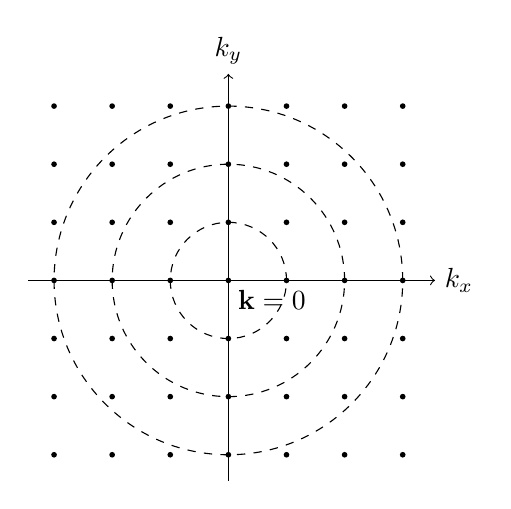
\begin{tikzpicture}[scale=0.82]
\draw[->] (-3.1,0) -- (3.2,0) node[right] {$k_x$};
\draw[->] (0,-3.1) -- (0,3.2) node[above] {$k_y$};
\draw[dashed] (0,0) circle (0.9);
\draw[dashed] (0,0) circle (1.8);
\draw[dashed] (0,0) circle (2.7);
\foreach \x in {-3,-2,-1,0,1,2,3}{
  \foreach \y in {-3,-2,-1,0,1,2,3}{
    \fill (0.9*\x,0.9*\y) circle (1.25pt);
  }
}
\node[below right] at (0,0) {$\mathbf{k}=0$};
\end{tikzpicture}
\caption{حالات الزخم المنفصلة والأغلفة متساوية الطاقة للجسيمات في صندوق دوري محدود.}
\end{figure}

بالنسبة إلى جسيم غير نسبي،
\begin{equation}
E_{\mathbf{k}}=\frac{\mathbf{k}^2}{2m},
\end{equation}
ومن ثم فإن الحالة الأدنى طاقة هي \(\mathbf{k}=0\). ضع \(N\) بوزونات متماثلة في الصندوق وابحث عن الحالة القاعية متعددة الجسيمات. يدخل البوزون الأول في حالة الزخم الصفري. ويمكن للثاني أن يدخل الحالة نفسها، وكذلك الثالث وكل بوزون تالٍ. ومن ثم تشغل جميع \(N\) بوزونات \(\mathbf{k}=0\).

هذا تكاثف بوزوني: عدد كبير من الجسيمات المتماثلة يشغل الحالة نفسها أحادية الجسيم، وهي هنا الحالة الأدنى طاقة. دالة الموجة ذات الزخم الصفري ثابتة مكانيًا وتمتد في الصندوق كله. وهي لا تُمَوْضِع أي بوزون بعينه عند موضع محدد؛ ولذلك يكون موضع كل بوزون غير متيقن بالمقابل. وعندما يصبح الإشغال كبيرًا، تبني دالة الموجة المشتركة سعة حقلية عيانية، ويزداد سلوك الحقل شبهاً بحقل كلاسيكي.

الحالة القاعية الفرميونية مختلفة تمامًا. تجاهل اللف المغزلي في الوقت الراهن، بحيث تمثل كل نقطة زخم حالة متاحة واحدة. يدخل الفرميون الأول في \(\mathbf{k}=0\)، لكن فرميونًا متماثلًا ثانيًا لا يمكنه الانضمام إليه. ويجب أن تشغل الجسيمات التالية غلاف الطاقة الأدنى التالي. ففي رسم ثنائي الأبعاد توجد أربع نقاط شبكية غير منعدمة هي الأقرب ومتساوية في الطاقة؛ وفي ثلاثة أبعاد توجد ست. وبعد شغل تلك الحالات، يجب أن تدخل الجسيمات اللاحقة أغلفة متعاقبة.

لأن الطاقة تتناسب مع مربع المسافة من الأصل في فضاء الزخم، فإن تصغير الطاقة الكلية يعني رصَّ النقاط المشغولة على أقرب ما يمكن حول \(\mathbf{k}=0\) كما يسمح به مبدأ الاستبعاد. ومع وجود عدد كبير من الفرميونات، تقارب المنطقة المشغولة كرة. وحدُّها هو سطح فيرمي، وداخلها هو بحر فيرمي، والمنطقة الممتلئة كاملة هي كرة فيرمي. وعند حجم منتهٍ يكون الحد مسننًا قليلًا لأن النقاط المتاحة تشكل شبكة، لكن هذه التفصيلة تصبح مهملة في نظام كبير.

\begin{figure}
\centering
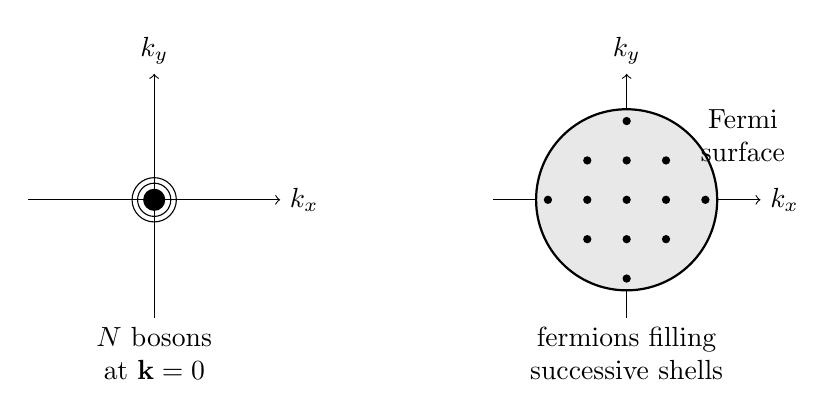
\begin{tikzpicture}[scale=1.0]
\begin{scope}[xshift=-3.0cm]
\draw[->] (-1.6,0) -- (1.6,0) node[right] {$k_x$};
\draw[->] (0,-1.5) -- (0,1.6) node[above] {$k_y$};
\fill (0,0) circle (4pt);
\draw (0,0) circle (6pt);
\draw (0,0) circle (8pt);
\node[align=center] at (0,-1.95) {$N$ bosons\\at $\mathbf{k}=0$};
\end{scope}
\begin{scope}[xshift=3.0cm]
\draw[->] (-1.7,0) -- (1.7,0) node[right] {$k_x$};
\draw[->] (0,-1.5) -- (0,1.6) node[above] {$k_y$};
\fill[gray!18] (0,0) circle (1.15);
\draw[thick] (0,0) circle (1.15);
\fill (0,0) circle (1.5pt);
\fill (0.5,0) circle (1.5pt);
\fill (-0.5,0) circle (1.5pt);
\fill (0,0.5) circle (1.5pt);
\fill (0,-0.5) circle (1.5pt);
\fill (0.5,0.5) circle (1.5pt);
\fill (0.5,-0.5) circle (1.5pt);
\fill (-0.5,0.5) circle (1.5pt);
\fill (-0.5,-0.5) circle (1.5pt);
\fill (1,0) circle (1.5pt);
\fill (-1,0) circle (1.5pt);
\fill (0,1) circle (1.5pt);
\fill (0,-1) circle (1.5pt);
\node[right,align=center] at (0.82,0.82) {Fermi\\surface};
\node[align=center] at (0,-1.95) {fermions filling\\successive shells};
\end{scope}
\end{tikzpicture}
\caption{تتكاثف البوزونات في حالة الزخم الصفري، في حين تملأ الفرميونات حالات الزخم إلى الخارج حتى سطح فيرمي.}
\end{figure}

تملك الحالة القاعية الفرميونية طاقة أكبر بكثير من طاقة الحالة القاعية البوزونية المناظرة. فجميع البوزونات يمكنها أن تبقى عند زخم صفري، لكن معظم الفرميونات تُجبَر على الدخول في حالات ذات زخم غير صفري. وكلما أُضيفت فرميونات أكثر، ازداد أكبر زخم مشغول. وفوق ذلك، يحتوي الغلاف عند زخم كبير على نقاط شبكية أكثر مما يحتويه غلاف قريب من الأصل. ولذلك تضم كرة فيرمي كبيرة كثيرًا من الجسيمات عند زخم معتبر، وعددًا قليلًا فقط في حالات الزخم الأدنى.

ويستمر هذا التباين في الحالات المثارة. فبالنسبة إلى البوزونات، تُحصَل الإثارة الأولى بإخراج أي بوزون واحد من المتكاثف ووضعه في أول حالة مثارة أحادية الجسيم:
\begin{equation}
(N,0,0,\ldots)\longrightarrow (N-1,1,0,\ldots).
\end{equation}
ولا فرق أيُّ بوزون يُنقل؛ فالجسيمات متماثلة. ويمكن تكوين إثارات أعلى بعدة طرائق. فبحسب تباعد المستويات، يمكن وضع بوزون واحد في مستوى أعلى أو وضع بوزونين في المستوى المثار الأول. وتعني إثارة النظام البوزوني رفع جسيمات من المتكاثف إلى حالات أعلى طاقة.

أما بالنسبة إلى الفرميونات، فلا يمكن نقل أي جسيم إلى نقطة أخرى داخل كرة فيرمي الممتلئة، لأن كل نقطة من هذا النوع مشغولة بالفعل. ومن الممكن أخذ فرميون من عمق البحر ووضعه فوق السطح، لكن ذلك يكلّف مقدارًا كبيرًا من الطاقة. وأقل الإثارات كلفةً تأخذ فرميونًا من موضع يقع مباشرة داخل سطح فيرمي وتنقله إلى حالة غير مشغولة تقع مباشرة خارجه. ولا يملك الإلكترون المرفوع إلا طاقة صغيرة فوق السطح، كما أن الحالة الشاغرة التي يتركها خلفه تقع على مسافة صغيرة فقط في الطاقة تحته.

\begin{figure}
\centering
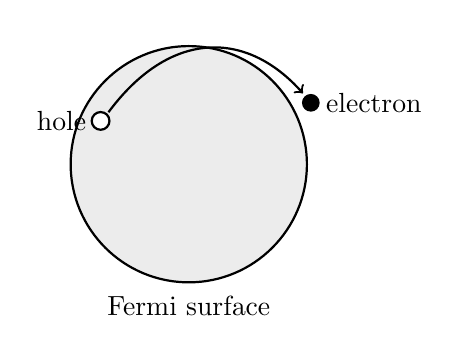
\begin{tikzpicture}[scale=1.0]
\fill[gray!15] (0,0) circle (1.5);
\draw[thick] (0,0) circle (1.5);
\draw[fill=white,thick] (-1.12,0.55) circle (3.2pt);
\fill (1.55,0.78) circle (3.2pt);
\draw[->,thick] (-1.02,0.66) .. controls (-0.25,1.7) and (0.72,1.72) .. (1.45,0.9);
\node[left] at (-1.18,0.55) {hole};
\node[right] at (1.62,0.78) {electron};
\node[below] at (0,-1.55) {Fermi surface};
\end{tikzpicture}
\caption{إثارة فرميونية منخفضة الطاقة ترفع إلكترونًا عبر سطح فيرمي وتخلّف وراءه ثقبًا.}
\end{figure}

\section{الثقوب والإثارات منخفضة الطاقة}

لتوضيح شحنة الثقب على نحو ملموس، تخيل أن الصندوق يحتوي شحنة موجبة موزعة بانتظام في حجمه كله. وفي المادة تأتي تلك الشحنة الموجبة في نهاية المطاف من البروتونات في الأنوية، لكن التوزيع المنتظم يُبقي النموذج بسيطًا. أضف عددًا كافيًا من الإلكترونات لمعادلة الخلفية. وفي الحالة القاعية تملأ تلك الإلكترونات كرة فيرمي.

إن رفع إلكترون واحد من أسفل سطح فيرمي إلى أعلاه لا يغيّر الشحنة الكلية للصندوق. فهو يخلق إلكترونًا ذا شحنة سالبة فوق السطح ويترك شحنة سالبة مفقودة تحته. ولذلك يمكن التعامل مع الإلكترون المفقود على أنه إثارة موجبة الشحنة: ثقب.

\begin{classroomqa}
\lecturetimestamp{01:31:38}
\audiencequestion{هل للثقب الواقع تحت سطح فيرمي طاقة سالبة؟}
\lecturerresponse{لا. الثقب إثارة فوق الحالة القاعية متعددة الأجسام، لذا فإن طاقة إثارته موجبة. وتتطلب إزالة إلكترون مشغول من تحت سطح فيرمي مقدارًا موجبًا من الطاقة عندما تُقاس الطاقات بالنسبة إلى ذلك السطح.}
\end{classroomqa}

لتكن طاقة الإلكترون المنزوع \(\varepsilon<\varepsilon_F\)، ولتكن طاقة الإلكترون المرفوع \(\varepsilon'>\varepsilon_F\). ويمكن فصل الطاقة المزوَّدة إلى فرقين موجبين في الطاقة عن سطح فيرمي.\footnote{يُذكر الفاصلان كلٌّ على حدة؛ والمساواة الموجزة المعروضة هنا هي إعادة تركيب مكافئة جبريًا.}
\begin{equation}
\Delta E
=\varepsilon'-\varepsilon
=(\varepsilon'-\varepsilon_F)+(\varepsilon_F-\varepsilon).
\end{equation}
ويُسنَد الإسهام الأول طبيعيًا إلى الإلكترون فوق سطح فيرمي، بينما يُسنَد الثاني إلى الثقب تحته:
\begin{equation}
E_{\mathrm{electron}}=\varepsilon'-\varepsilon_F>0,
\qquad
E_{\mathrm{hole}}=\varepsilon_F-\varepsilon>0.
\end{equation}
يحمل الإلكترون شحنة سالبة، ويحمل الثقب شحنة موجبة.

قد يهبط إلكترون فوق سطح فيرمي لاحقًا إلى ثقب متاح. وعندئذ تنخفض طاقته، لذا يجب أن يحمل الإشعاع الطاقة المنطلقة بعيدًا. ويمكن وصف الحدث بأنه هبوط إلكترون إلى حالة أدنى غير مشغولة مع إصدار فوتون واحد أو أكثر. وبصورة مكافئة، يمكن القول إن إلكترونًا وثقبًا يفني أحدهما الآخر إلى إشعاع. والثقب ليس مكوِّنًا أساسيًا إضافيًا في الصندوق؛ بل هو غياب في الحالة الممتلئة متعددة الإلكترونات. ومع ذلك فإن طاقته وشحنته تجعل من المفيد التعامل معه على أنه إثارة شبيهة بالجسيم.

\begin{classroomqa}
\lecturetimestamp{01:36:52}
\audiencequestion{هل يعني رفع إلكترون نقله من نقطة شبكية إلى أخرى في فضاء الزخم؟}
\lecturerresponse{إنه يعني نقل الإلكترون من مستوى طاقة إلى آخر. وبالنسبة إلى الجسيمات الحرة في الصندوق، تُعيّن شبكة الزخم تلك المستويات، لكن الفكرة نفسها لا تعتمد على شبكة في فضاء الزخم. وفي الذرة تتركز الشحنة الموجبة في النواة. وتشغل الإلكترونات أدنى المستويات الذرية المتاحة، ويمكن لفوتون أن يرفع إلكترونًا واحدًا إلى مستوى مثار، تاركًا شاغرًا في المستوى الذي جاء منه. وهذا الشاغر هو النظير الذري للثقب.}
\end{classroomqa}

وفي الصندوق، يحوّل امتصاص الفوتون كذلك طاقة الفوتون إلى إلكترون فوق سطح فيرمي وثقب تحته. وفي الذرة، تصف اللغة نفسها الإلكترون المثار مع الشاغر الذي يتركه بين المستويات الدنيا المشغولة.

\begin{classroomqa}
\lecturetimestamp{01:39:16}
\audiencequestion{هل يمكن أن يمتص إلكترون في أي مكان من كرة فيرمي فوتونًا منخفض الطاقة؟}
\lecturerresponse{لا. فإذا كان الإلكترون عميقًا في بحر فيرمي، كانت كل الحالات القريبة منه مشغولة بالفعل، ولا يستطيع فوتون منخفض الطاقة رفعه حتى يصل إلى حالة غير مشغولة فوق السطح. والإلكترونات القريبة بما يكفي من سطح فيرمي وحدها هي التي تملك حالات خالية متاحة ضمن مجال طاقة الفوتون. ويمكن لفوتون ذي طاقة كافية أن يثير إلكترونًا من عمق البحر.}
\end{classroomqa}

لذلك يحدَّد المقطع العرضي للامتصاص منخفض الطاقة بسطح بحر فيرمي لا بحجمه كله. فالإلكترونات العميقة في البحر محجوبة عن إجراء انتقالات صغيرة؛ أما الإلكترونات الواقعة مباشرة تحت السطح فيمكن نقلها إلى ما فوقه مباشرة.

\begin{classroomqa}
\lecturetimestamp{01:40:42}
\audiencequestion{ما الذي يمنع الإلكترونات من التآثر مباشرة بعضها مع بعض، من دون فوتون ساقط؟}
\lecturerresponse{لا شيء. يجري إهمال تآثرات الإلكترون--الإلكترون في هذا النموذج البسيط، لأن تضمينها يجعل صورة بحر فيرمي أكثر تعقيدًا. وفي هذا التقريب الأول للفلز، يُعامَل تأثيرها الفعّال على أنه ضعيف بما يكفي بحيث يمكن تجاهله عادةً.}
\end{classroomqa}

\begin{classroomqa}
\lecturetimestamp{01:41:10}
\audiencequestion{ماذا يحدث إذا حمل فوتون واحد طاقة تكفي لإثارة عدة إلكترونات؟}
\lecturerresponse{من حيث المبدأ، كل عملية تنسجم مع قوانين الانحفاظ ممكنة. ويمكن للفوتون أن يخلق أكثر من زوج إلكترون--ثقب واحد: فإثارة إلكترونين تترك أيضًا ثقبين. وتخلق مثل هذه العملية عددًا أكبر من الإثارات، وهي عمومًا أقل احتمالًا من استخدام الطاقة لإثارة إلكترون واحد بدرجة أشد كثيرًا.}
\end{classroomqa}

\begin{classroomqa}
\lecturetimestamp{01:42:06}
\audiencequestion{هل يمكن امتصاص فوتونين معًا عندما لا يستطيع أيٌّ من الفوتونين منفردًا إحداث الإثارة؟}
\lecturerresponse{نعم. الامتصاص احتمالي، ويمكن أن تحدث عملية ثنائية الفوتون عندما تبلغ طاقة الفوتونين معًا إثارةً متاحة، رغم أن طاقة كل فوتون على حدة تبقى دون الطاقة المطلوبة. وإذا كان الضوء المتاح يحمل طاقة قليلة جدًا بحيث لا يصل إلى أي إثارة مسموح بها، فإنه يمر عبر النظام في معظمه.}
\end{classroomqa}

\editorialnote{يربط نقاش موجز عند هذه النقطة الإشعاع الممتص بالحركة الجماعية للإلكترونات، لكن تفاصيله الجوهرية غير قابلة للاستعادة. والعبارة الوحيدة الموثوقة هي أن هذه الاستجابة الجماعية أعقد من صورة الجسيم المفرد--الثقب.}

\begin{classroomqa}
\lecturetimestamp{01:43:49}
\audiencequestion{لماذا تُسمى تآثرات الإلكترون--الإلكترون ضعيفةً مع أن جميع الإلكترونات تحمل الشحنة السالبة نفسها؟}
\lecturerresponse{الإلكترونات مغمورة في الخلفية الموجبة المعوِّضة. وهذه الخلفية تحجب شحنة الإلكترون وتقلل التآثر الفعال في هذا الإطار المبسَّط. والتآثر ليس منعدمًا؛ فمعالجته تتطلب استجابة الحجب الخاصة بالوسط.}
\end{classroomqa}

\begin{classroomqa}
\lecturetimestamp{01:44:41}
\audiencequestion{هل ستُناقش ظاهرة الحجب لاحقًا؟}
\lecturerresponse{نعم. الحجب مهم، لكنه مؤجل إلى أن يمكن تناول النظام المتآثر على نحو أكمل.}
\end{classroomqa}

\section{بحر فيرميوني أحادي البعد والجسيمات المضادة}

يقود بناء الثقب إلى الجسيمات المضادة. ويمكن نقل البنية المنطقية نفسها من إلكترونات المادة إلى حقل كمومي نسبي وفراغه. وتستخدم أبسط صيغة بُعدًا مكانيًا واحدًا وحقلًا فيرميونيًا عديم الكتلة \(\psi(x,t)\). وفي وحدات تكون فيها سرعة الضوء مساويةً للواحد، تكون علاقتا التشتت الخطيّتان الممكنتان هما
\begin{equation}
\omega=k,
\qquad\text{or}\qquad
\omega=-k.
\end{equation}
وسنعالج الفرع الأول صراحةً.

\editorialnote{يتناوب الحوار الختامي على تعيينات غير متوافقة للجسيمات. أما النموذج الموثوق فهو حقل فيرميوني مبسَّط غير محدد وعديم الكتلة في بعد مكاني واحد، ومقيَّد باتجاه انتشار واحد.}

بالنسبة إلى موجة مستوية
\begin{equation}
\psi(x,t)=e^{i(kx-\omega t)},
\end{equation}
تكون المشتقات
\begin{equation}
\frac{\partial\psi}{\partial t}=-i\omega\psi,
\qquad
\frac{\partial\psi}{\partial x}=ik\psi.
\end{equation}
وعليه، فإن العلاقة \(\omega=k\) تكافئ معادلة الحقل من الرتبة الأولى
\begin{equation}
\frac{\partial\psi}{\partial t}
=-\frac{\partial\psi}{\partial x}.
\end{equation}

\begin{figure}
\centering
\includegraphics[width=0.72\textwidth]{lecture_05_figure_05.png}
\caption{البدء بمعادلة الحقل من الرتبة الأولى التي تحقق موجاتها المستوية العلاقة \(\omega=k\).}
\lectureframe{01:47:22}
\end{figure}

أي تابع من الشكل \(f(x-t)\) يحقق هذه المعادلة ويتحرك إلى اليمين. وعكس الإشارة يعطي
\begin{equation}
\frac{\partial\psi}{\partial t}
=+\frac{\partial\psi}{\partial x},
\end{equation}
وحلولها من الشكل \(f(x+t)\) تتحرك إلى اليسار. وكل معادلة من الرتبة الأولى منهما تنتقي اتجاهًا واحدًا فقط للحركة. ولنأخذ الحقل فيرميونيًا، ولأجل حجة الثقب نفترض أن جسيماته تحمل شحنة كهربائية.

ينطوي الفرع \(\omega=k\) على صعوبة فورية. إذ يمكن أن يكون عدد الموجة \(k\) سالبًا، وبالتالي يمكن أن تكون \(\omega\) سالبةً أيضًا. وبما أن \(\omega\) تمثل الطاقة في هذه الوحدات، فإن الطيف الخطي يحتوي حالات ذات طاقة موجبة وأخرى ذات طاقة سالبة:
\begin{equation}
E=\omega=k.
\end{equation}

\begin{figure}
\centering
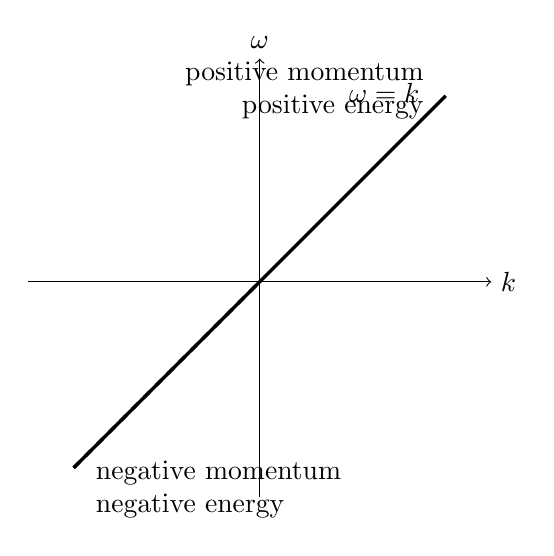
\begin{tikzpicture}[scale=1.05]
\draw[->] (-2.8,0) -- (2.8,0) node[right] {$k$};
\draw[->] (0,-2.6) -- (0,2.7) node[above] {$\omega$};
\draw[very thick] (-2.25,-2.25) -- (2.25,2.25);
\draw[very thick,dashed] (-2.25,-2.25) -- (0,0);
\node[above left] at (2.05,2.05) {$\omega=k$};
\node[below right,align=left] at (-2.1,-2.05) {negative momentum\\negative energy};
\node[above left,align=right] at (2.1,1.85) {positive momentum\\positive energy};
\end{tikzpicture}
\caption{طيف الفرع الواحد \(\omega=k\)، ويقع نصفه ذو الطاقة السالبة عند \(k<0\).}
\end{figure}

لا يمكن لفراغ خالٍ عادي أن يكون الحالة القاعية لمثل هذه النظرية. إذ يمكن لفيرميون ذي طاقة موجبة أن يشع فوتونًا ويهبط إلى حالة أدنى. ولا شيء يجبره على التوقف عند الصفر: إذ يمكنه أن يواصل الهبوط إلى حالات ذات طاقة سالبة، وأن يصدر مزيدًا من الإشعاع، وأن يهبط بلا حد. وتظهر الطاقة التي يفقدها الفيرميون في حقل الإشعاع. ولذلك فإن طيفًا غير محدود من أسفل لا يعطي فراغًا عاديًا مستقرًا.

يوفر استبعاد فيرمي نقطة انطلاق مختلفة. املأ كل حالة أحادية الجسيم ذات طاقة سالبة، حتى طاقة الصفر، بفيرميون واحد. ولا يستطيع أي فيرميون إضافي أن يهبط إلى تلك الحالات لأن كلًا منها مشغول بالفعل. وإضافة فيرميون آخر ذي طاقة سالبة أمر مستحيل، في حين أن إضافة فيرميون ذي طاقة موجبة ترفع الطاقة. ولذلك يمكن اعتبار بحر الطاقة السالبة الممتلئ تمامًا الحالة القاعية للنظام عديد الأجسام، وتسميته الفراغ.

\begin{figure}
\centering
\resizebox{\linewidth}{!}{%
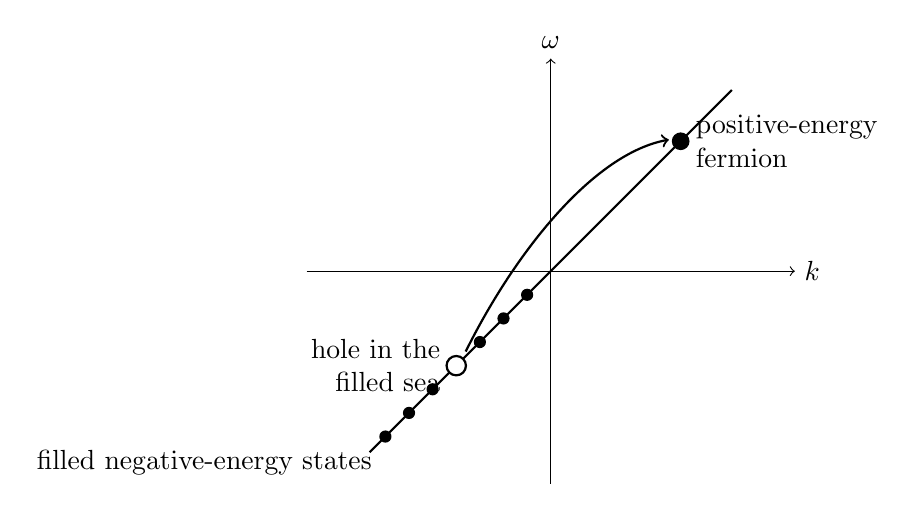
\begin{tikzpicture}[scale=1.0]
\draw[->] (-3.1,0) -- (3.1,0) node[right] {$k$};
\draw[->] (0,-2.7) -- (0,2.7) node[above] {$\omega$};
\draw[thick] (-2.3,-2.3) -- (2.3,2.3);
\foreach \p in {-2.1,-1.8,-1.5,-1.2,-0.9,-0.6,-0.3}{
  \fill (\p,\p) circle (2.2pt);
}
\draw[fill=white,thick] (-1.2,-1.2) circle (3.5pt);
\fill (1.65,1.65) circle (3.2pt);
\draw[->,thick] (-1.08,-1.02) .. controls (-0.45,0.25) and (0.55,1.5) .. (1.5,1.67);
\node[left,align=right] at (-1.28,-1.2) {hole in the\\filled sea};
\node[right,align=left] at (1.72,1.65) {positive-energy\\fermion};
\node[below left] at (-2.15,-2.15) {filled negative-energy states};
\end{tikzpicture}%
}
\caption{بحر الطاقة السالبة الممتلئ وإثارة تتكون برفع فيرميون واحد إلى طاقة موجبة.}
\end{figure}

أبسط إثارة تنزع فيرميونًا واحدًا من بحر الطاقة السالبة وترفعه إلى حالة ذات طاقة موجبة. والفيرميون المرفوع جسيم عادي ذو طاقة موجبة. والشغور الذي يتركه في البحر هو إثارة ثانية، أي ثقب. وإذا كان الفيرميون المنزوع ذا شحنة سالبة، كان الثقب ذا شحنة موجبة.

للثقب أيضًا زخم موجب في هذا المثال ذي الفرع الواحد. فإذا كان الفيرميون المفقود يشغل حالةً ذات زخم \(k_-<0\)، فإن إزالته تغير الزخم الكلي بمقدار
\begin{equation}
p_{\mathrm{hole}}=-k_->0.
\end{equation}
وهذا عجز في الزخم السالب. ومن ثم تتألف الإثارة من فيرميون ذي طاقة موجبة وشحنة سالبة، وثقب ذي طاقة موجبة وشحنة موجبة. وكلاهما يحمل زخمًا موجبًا، وعلى الفرع \(\omega=k\) يتحركان إلى اليمين.

في نظرية الإلكترون الكاملة، الثقب ذو الشحنة الموجبة هو البوزيترون. وقد نظر ديراك أولًا في مطابقة الثقب مع البروتون. ويتطلب هذا البناء أن تكون للجسيم ولجسيمه المضاد الكتلة نفسها. والثقب جسيم متميز له كتلة الإلكترون وشحنة كهربائية معاكسة. وهذا هو التفسير الأساسي للجسيم--الجسيم المضاد الذي قاد إليه طيف الطاقة السالبة.

لا يمكن تطبيق وسيلة الإنقاذ نفسها على البوزونات. فالحالة البوزونية تقبل عددًا اعتباطيًا من الجسيمات، لذلك لا توجد طريقة لملء مستوى ذي طاقة سالبة مرةً واحدة ومنع إشغال إضافي له. إذ يمكن دائمًا إضافة مزيد من البوزونات إلى ذلك المستوى، مما يخفض الطاقة مرة بعد مرة:
\begin{equation}
\begin{aligned}
\text{fermionic mode: }&n=0\ \text{or}\ 1,\\
\text{bosonic mode: }&n=0,1,2,\ldots .
\end{aligned}
\end{equation}
وسيظل النظام البوزوني المقترح بلا حالة قاعية. وفي هذا البناء الابتدائي، تعتمد استقرارية البحر الممتلئ على استبعاد فيرمي على وجه التحديد.

هذه المعادلة الأحادية البعد ليست إلا نسخة مبسطة من معادلة ديراك. فحقلها عديم الكتلة، ويتحرك بسرعة الضوء، وينتشر في اتجاه واحد فقط. ويجب أن تستوعب الصيغة الأكثر اكتمالًا لمعادلة ديراك اتجاهات الحركة المفقودة وسائر بنية الجسيم النسبي. وتؤجَّل هذه الصيغة الأكمل، مع معالجة الجسيمات المضادة في الحقول البوزونية.
